\section{Repeated Pulse Delay MLE}
\label{sec:Repeated-Pulse-Delay-Estimation}

We now examine the same problem of~\Cref{sec:Single-Pulse-Delay-Estimation}, but this time we assume that the transmitted signal \(t\mapsto s(t)\) is a repeated pulse. We keep the assumption that the detected signal retains the same shape and extension as in~\eqref{eq:thetriade}, but instead of~\eqref{eq:rectmodel} we have:
\begin{equation}
s(t)=\sum_{m=0}^{M-1}\operatorname{rect}_{(nT_s)}\left(t-mQT_s\right),
\label{eq:thesponge}
\end{equation}
where \(M\) is the number of cycles of the transmitted signal~\eqref{eq:thesponge}, \(n \in \mathbb{Z}_{\geq1}\) is the length in time slots of the rectangular function \(t\mapsto\operatorname{rect}_{(nT_s)}(t)\), \(Q\in \mathbb{Z}_{> n}\) and the duty cycle of the signal can be seen as \((nT_s)/(QT_s)=n/Q\) as shown in~\Cref{fig:repeated}. Like in~\Cref{sec:Single-Pulse-Delay-Estimation}, the number of photons arriving in each time slot \(i\) is
\begin{equation}
\begin{aligned}
x_r[i]
& \sim \operatorname{Poi}\left(\psi_{i,r}(\delta_r)\right),
\label{eq:observationsx}
\end{aligned}
\end{equation}
where
\begin{equation}
\psi_{i,r}(\delta_r)
= \int_{iT_s}^{(i+1)T_s} \left[ \lambda_{b,r}+\lambda_{s,r} \, s(t-\delta_{r}) \right] \di t
= \lambda_{b,r} T_s+\lambda_{s,r}\, S_i\left(\delta_r\right),
\end{equation}
and
\begin{equation}
S_i(\delta_r) = \int_{iT_s}^{(i+1)T_s} s(t-\delta_r) \di t.
\end{equation}

\begin{figure}[!b]
\centering
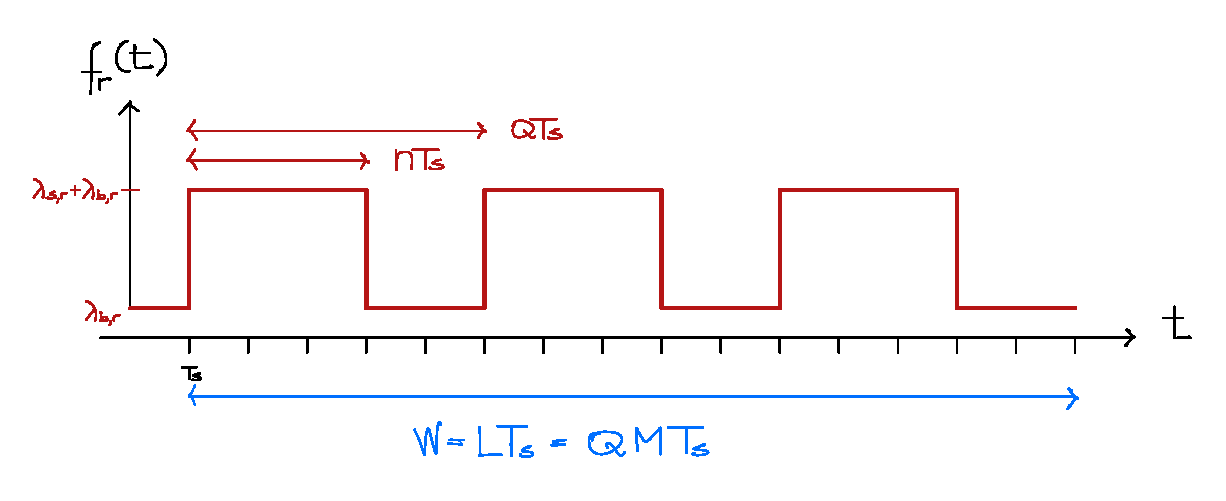
\includegraphics[
  width=0.9\textwidth,
  keepaspectratio,
  clip,
]{figs/repeatedpulse.pdf}
\caption[]{Plot of the detected pulse~\eqref{eq:thesponge}.}
\label{fig:repeated}
\end{figure}

The number of total observations is \(L=QM\) i.e. \(i\in\{0,\ldots,QM-1\}\), and are going to make the critical assumption that, in order to estimate the total time delay \(\delta_r\), the system is capable of disregarding the time when the receiver is completely idle and take into consideration for the estimate only the portion of time where the repeated pulse is detected. Furthermore, we assume that the number of cycles \(M\) is large enough that we can consider~\eqref{eq:thesponge} to be fully periodic in our analysis, effectively disregarding the edge case when the signal is about to reach the idle receiver. In mathematical terms:
\begin{equation}
s(t)=\sum_{m=0}^{M-1}\operatorname{rect}_{(nT_s)}\left(t-mQT_s\right)
\approx\operatorname{rect}_{(nT_s)} \left(t\,\text{mod}\, QT_s\right).
\label{eq:assumtions}
\end{equation}

\noindent
Given these assumptions, observations~\eqref{eq:observationsx} are merged into a discrete vector of length \(Q\):
\begin{equation}
y_r[k]=\sum_{m=0}^{M-1}x_r[k+mQ] \quad k\in\{0,\ldots,Q-1\}.
\label{eq:aparently}
\end{equation}
Since we assume observations~\eqref{eq:observationsx} to be independent Poisson random variables, we then know that also \(y_r[k]\) with \(k\in\{0,\ldots,Q-1\}\) are also Poisson random variables:
\begin{equation}
y_r[k]\sim
\operatorname{Poi}
\left(\xi_{k,r}(\delta_r)\right),
\end{equation}
where
\begin{equation}
\begin{aligned}
\xi_{k,r}(\delta_r)
& = \sum_{m=0}^{M-1}\psi_{(k+mQ),r}(\delta_r)\\
& = \sum_{m=0}^{M-1}\int_{(k+mQ)T_s}^{(k+mQ+1)T_s} \left[ \lambda_{b,r}+\lambda_{s,r} \, s(t-\delta_{r}) \right] \di t\\
& = M\lambda_{b,r} T_s+\lambda_{s,r} \sum_{m=0}^{M-1}\int_{(k+mQ)T_s}^{(k+mQ+1)T_s}  s(t-\delta_{r}) \di t\\
& \overset{\text{(a)}}{=}  M\lambda_{b,r} T_s+\lambda_{s,r} \sum_{m=0}^{M-1}\int_{(k+mQ)T_s}^{(k+mQ+1)T_s}  \operatorname{rect}_{(nT_s)} \left((t-\delta_r) \,\text{mod}\, QT_s\right) \di t\\
& \overset{\text{(b)}}{=}  M\lambda_{b,r} T_s+M\lambda_{s,r} \int_{kT_s}^{(k+1)T_s}  \operatorname{rect}_{(nT_s)} \left((t-\delta_r) \,\text{mod}\, QT_s\right) \di t\\
\end{aligned}
\label{eq:position}
\end{equation}
and where in step (a) we used assumption~\eqref{eq:assumtions} and in step (b) we simplified the summation over a single period \(QT_s\).

\subsection{ML Estimation Repeated Pulse}\label{sub:MLestimation2}

\noindent
Like~\Cref{sub:MLestimation1} we first look at a \textbf{single receiving antenna first}, denoting the \textbf{total time delay} \(\delta_r\) with \(\delta\) and the number of photons arriving at the ``merged'' time slot \(k\), \(y_r[k]\) simply with \(y_k\). The observation vector is then \(\mathbf{y}=(y_0,\ldots,y_{Q-1})\) and the log-likelihood of these \(Q\) observations is:
\begin{equation}
\begin{aligned}
\ell(\delta ; \mathbf{y})
= & \log p_{\textbf{x} \mid \delta}\left(x_0, \ldots,y_{Q-1} \mid \delta\right)\\
= & \sum_{k=0}^{Q-1} \log p_{y_k \mid \delta}\left(y_k \mid \delta\right) \\
= & \sum_{k=0}^{Q-1} y_k \log \left( \xi_k(\delta)\right) -\xi_k(\delta)-\log \left(y_{k}!\right).
\end{aligned}
\end{equation}
We note from~\eqref{eq:position} that:
\begin{equation}
\sum_{k=0}^{Q-1}\xi_k(\delta)
=QM\lambda_{b,r} T_s+M\lambda_{s,r} \int_{0}^{QT_s}  \operatorname{rect}_{(nT_s)} \left((t-\delta_r) \,\text{mod}\, QT_s\right) \di t
\end{equation}
and
\begin{equation}
\sum_{k=0}^{Q-1}\log \left(y_{k}!\right),
\end{equation}
are constants with respect to \(\delta\).

\noindent
Therefore, like in~\eqref{eq:sweetsix}, we have:
\begin{equation}
\begin{aligned}
\delta_{\mathrm{ML}} 
=\underset{\delta}{\argmax} 
\sum_{k=0}^{Q-1} y_k \log \left( \xi_k(\delta)\right).
\end{aligned}
\end{equation}

\noindent
Like in~\Cref{sub:MLestimation1}, the log-likelihood is only differentiable and concave in the open interval \((kT_s,(k+1)T_s)\) corresponding to the merged time slot \(k,\;\forall k\in\{0,\ldots,Q-1\}\).

\noindent
We then take the derivative with the log-likelihood over the interval \(\delta \in(kT_s,(k+1)T_s)\):
\begin{equation}
\begin{aligned}
\frac{\partial}{\partial \delta} \ell(\delta ; \mathbf{x})
&= \frac{\partial}{\partial \delta}\sum_{k=0}^{Q-1} y_k \log \left( \xi_k(\delta)\right)
=  \sum_{k=0}^{Q-1}y_k\frac{ \frac{\partial}{\partial \delta}\xi_k(\delta)}{\xi_k(\delta)}\\
&= y_{k+n} \frac{M\lambda_s}{\left(M\lambda_s \delta-k M\lambda_s T_s\right)+M\lambda_b T_s}-y_k \frac{M\lambda_s}{\left(-M\lambda_s \delta+(k+1) M\lambda_s T_s\right)+M\lambda_b T_s}\\
&= \frac{y_{k+n}}{\left( \delta-k  T_s\right)+\frac{\lambda_b}{\lambda_s} T_s}- \frac{y_k}{\left(- \delta+(k+1)  T_s\right)+\frac{\lambda_b}{\lambda_s} T_s},
\end{aligned}
\label{eq:thesumming}
\end{equation}
which is exactly the same solution of~\eqref{eq:plutone}. From this we know that:
\begin{equation}
\begin{aligned}
\delta_{\mathrm{ML}, i}
&=T_s\left[\frac{y_{i+n}\left(i+1 +\frac{\lambda_b}{\lambda_s} \right)+y_i\left(i -\frac{\lambda_b}{\lambda_s} \right)}{y_i+y_{i+n}}\right],
\end{aligned} 
\end{equation}
and the final estimate is then found as the maximum between the interval estimates:
\begin{equation}
    \delta_{\mathrm{ML}}=\underset{i}{\argmax} \; \ell\left(\delta_{\mathrm{ML}, i} ; \mathbf{y}\right) \quad i\in\{0, \ldots, Q-1\}.
    \label{eq:estimatestupid}
\end{equation}
The Cramér-Rao Bound, the bias and the variance of the are the same as the ones found in~\Cref{sec:Single-Pulse-Delay-Estimation} only with \(y_r[k]\) as defined in~\eqref{eq:aparently} instead of \(x_r[k]\).